% https://es.overleaf.com/latex/templates/project-report/jpzczmpsdzwm

%%% Preamble
\documentclass[paper=leter, fontsize=11pt]{scrartcl}
\usepackage[utf8]{inputenc}
\usepackage[spanish,mexico]{babel}
\usepackage[T1]{fontenc}    % use 8-bit T1 fonts
\usepackage{lmodern}
\usepackage{hyperref}       % hyperlinks
\usepackage{lipsum}
\usepackage[square,numbers]{natbib}

\usepackage[protrusion=true,expansion=true]{microtype}	
\usepackage{amsmath,amsfonts,amsthm} % Math packages
\usepackage[pdftex]{graphicx}
\usepackage{url}
 
\usepackage{booktabs}
\usepackage[table,xcdraw]{xcolor}

\usepackage{tikz}
\usetikzlibrary{positioning,matrix, arrows.meta}

\usepackage{caption} 
\usepackage{subcaption}


\usepackage{listings}
\lstdefinestyle{mystyle}{ 
    basicstyle=\ttfamily\footnotesize,
    breakatwhitespace=false,         
    breaklines=true,                 
    captionpos=b,                    
    keepspaces=true,                 
    numbers=left,                    
    numbersep=5pt,                  
    showspaces=false,                
    showstringspaces=false,
    showtabs=false,                  
    tabsize=4
}

\lstset{style=mystyle}
\renewcommand{\lstlistingname}{Código}


\selectlanguage{spanish}
\usepackage[spanish,onelanguage,ruled]{algorithm2e}


%%% Custom sectioning
\usepackage{sectsty}
\allsectionsfont{\centering \normalfont\scshape}


%%% Custom headers/footers (fancyhdr package)
\usepackage{fancyhdr}
\pagestyle{fancyplain}
\fancyhead{}											% No page header
\fancyfoot[L]{}											% Empty 
\fancyfoot[C]{}											% Empty
\fancyfoot[R]{\thepage}									% Pagenumbering
\renewcommand{\headrulewidth}{0pt}			% Remove header underlines
\renewcommand{\footrulewidth}{0pt}				% Remove footer underlines
\setlength{\headheight}{13.6pt}


%%% Equation and float numbering
\numberwithin{equation}{section}		% Equationnumbering: section.eq#
\numberwithin{figure}{section}			% Figurenumbering: section.fig#
\numberwithin{table}{section}				% Tablenumbering: section.tab#


%%% Maketitle metadata
\newcommand{\horrule}[1]{\rule{\linewidth}{#1}} 	% Horizontal rule

%%% https://tex.stackexchange.com/a/118217
\usepackage{mathtools}
\DeclarePairedDelimiter\ceil{\lceil}{\rceil}
\DeclarePairedDelimiter\floor{\lfloor}{\rfloor}

\usepackage{amsmath}

\usepackage{tikz}

\title{
		%\vspace{-1in} 	
		\usefont{OT1}{bch}{b}{n}
		\normalfont \normalsize \textsc{Posgrado de Ingeniería de Sistemas} \\ [25pt]
		\horrule{0.5pt} \\[0.4cm]
		\huge Frecuencias \\
		\horrule{2pt} \\[0.5cm]
}
\author{
		\normalfont 								\normalsize
        Alberto Benavides\\[-3pt]		\normalsize
        \today
}
\date{}


%%% Begin document
\begin{document}
\maketitle

\section{Introducción}

Un análisis estadístico básico de un libro consiste en analizar la frecuencia de las palabras con que está escrito. Una guía bastante completa para lograrlo en R \cite{r} puede consultarse en \url{https://tinyurl.com/y64jld27}.

\section{Recursos}

El libro de Dracula \cite{dracula} se encuentra disponible de manera gratuita en el sitio de Project Gutemberg que alberga libros cuya propiedad intelectual ha caducado y, por lo tanto, se trata de obras que forman parte del dominio público. Se puede acceder a los textos planos de estas obras mediante la librería \texttt{gutembergr} \cite{gutenbergr} de R y la descomposición en palabras de la obra se facilita con el uso de \texttt{tidytext} \cite{tidytext} que, a su vez, utiliza para su funcionamiento la librería \texttt{dplyr} \cite{dplyr}. Existe un cuaderno de Jupyter \cite{jupyter} donde se trabajaron los datos disponible en \url{https://tinyurl.com/y3dp3ngl}.

\section{Preprocesamiento}
Después de obtenido el libro mediante la función \texttt{gutenberg\_download}, se analiza su contenido inicial y final con las funciones \texttt{head} y \texttt{tail}. Esto muestra la existencia de apartados introductorios y anexos que se escapan del contenido del libro en sí, por lo que se procede a remover del contenido esos elementos. Destaca aquí el uso de la función \texttt{grep} que permite identificar expresiones regulares y, en este caso, la ubicación del final del libro que coindice con las palabras ``THE END''.

\section{Resultados y análisis}
Una vez identificado y aislado el contenido del libro, se extraen las letras y palabras que contiene con la función \texttt{unnest\_tokens} de la librería \texttt{tidytext}. Luego se genera una tabla de frecuencias en orden descendiente por conteo de aparición de las diez letras y palabras más usadas mediante la función \texttt{order}. Dichas tablas se grafican en los diagramas de barras de las figuras \ref{letras} (p. \pageref{letras}) y \ref{palabras} (p. \pageref{palabras}).

\begin{figure}
    \centering
    \includegraphics[width=1\textwidth]{letras.eps}
    \caption{Diagrama de barras de las frecuencias de aparición de los caracteres más usados en el libro de \textit{Dracula}.}
    \label{letras}
\end{figure}

\begin{figure}
    \centering
    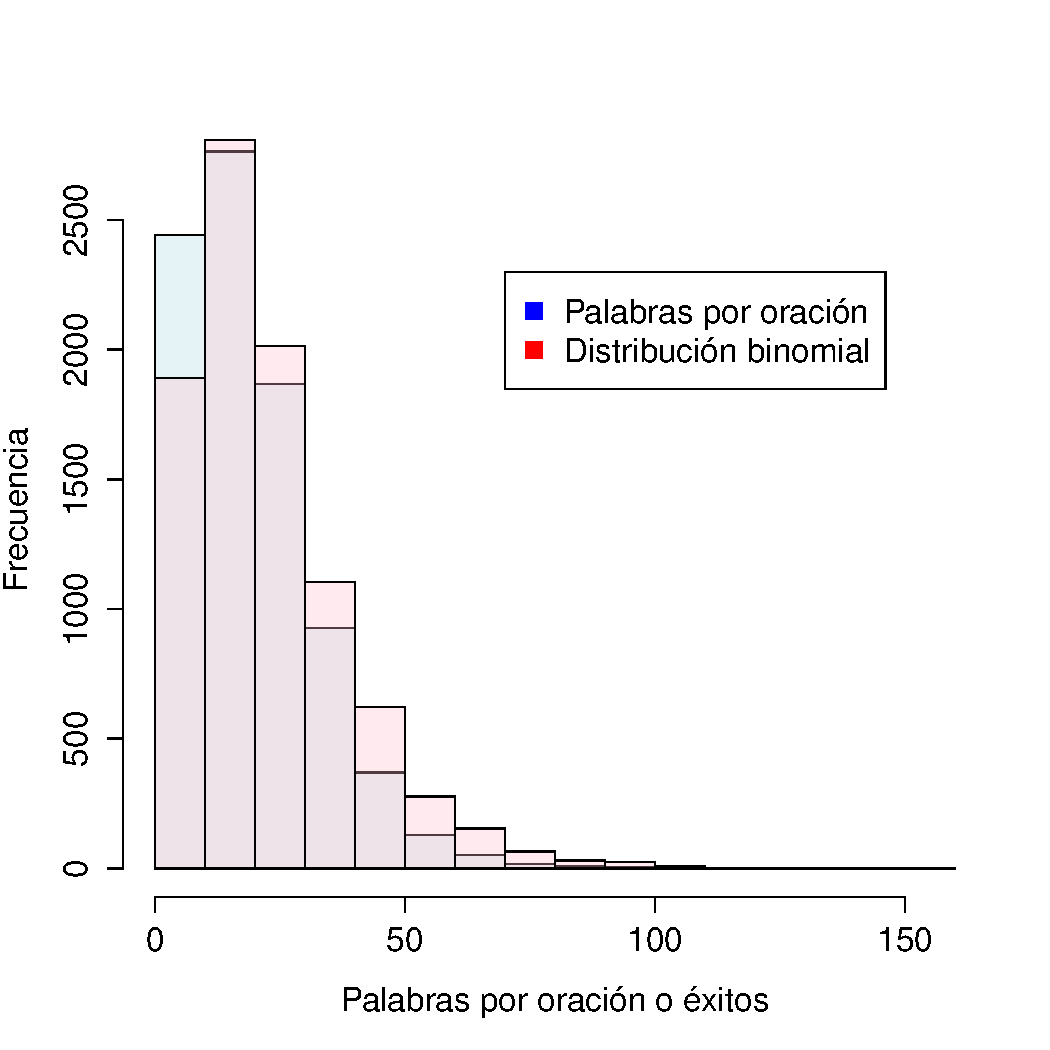
\includegraphics[width=1\textwidth]{palabras.eps}
    \caption{Diagrama de barras de las frecuencias de aparición de las palabras más usadas en el libro de \textit{Dracula}.}
    \label{palabras}
\end{figure}

En cuanto al contexto del libro, esta información no es muy relevante puesto que las palabras que aparecen se denominan palabras vacías (o stop words en ingl+es) que se refiere a palabras que en un idioma carecen de significado fuera de contexto (más información en \url{https://tinyurl.com/y2pr7kcb}). En español se incluyen todos las preposiciones, artículos y adverbios. Al eliminar estas palabras, se obtiene una lista de palabras más significativas cuya representación gráfica en una nube de palabras se puede consultar en la figura \ref{wc_palabras} (p. \pageref{wc_palabras}).

\begin{figure}
    \centering
    \includegraphics[width=1\textwidth]{wc_palabras.eps}
    \caption{Nube de palabras de las palabras más representativas de la obra \textit{Dracula}.}
    \label{wc_palabras}
\end{figure}

Asimismo, se hizo una animación de la frecuencia acumulada de las cincuenta palabras más significativas que aparecen en la obra a partir del porcentaje de avance de la misma, de uno en uno por ciento. Esta animación puede verse en \url{https://tinyurl.com/y2dnxrv8}.

Por último, se analizaron los \textbf{bigramas}, o sea las palabras que más comúnmente se encuentran seguidas a lo largo de la obra. Éstos se pueden obtener también con la función \texttt{unnest\_tokens(bigram, \ldots)} (existen dos tutoriales muy completos en \url{https://tinyurl.com/y5yzdxdm} y \url{https://tinyurl.com/y2qcvrcq}). El procedimiento consiste en encontrar los bigramas, eliminar aquéllos que contienen palabras vacías y realizar un conteo de los más significativos. Un grafo de estos bigramas con al menos diez apariciones puede observarse en la figura \ref{bigramas} (p. \pageref{bigramas}). Como puede obserarse, la mayoría de los bigramas formados pertenecen a nombres de personas o a títulos seguidos de nombres, por ejemplo ``Dr. Seward''. Aparte de estos bigramas, destacan los ``poor Lucy'' o ``dear Lucy'' personaje por el que podría arrojarse la suposición de que es tan querida como conmiserada durante la obra.

\begin{figure}
    \centering
    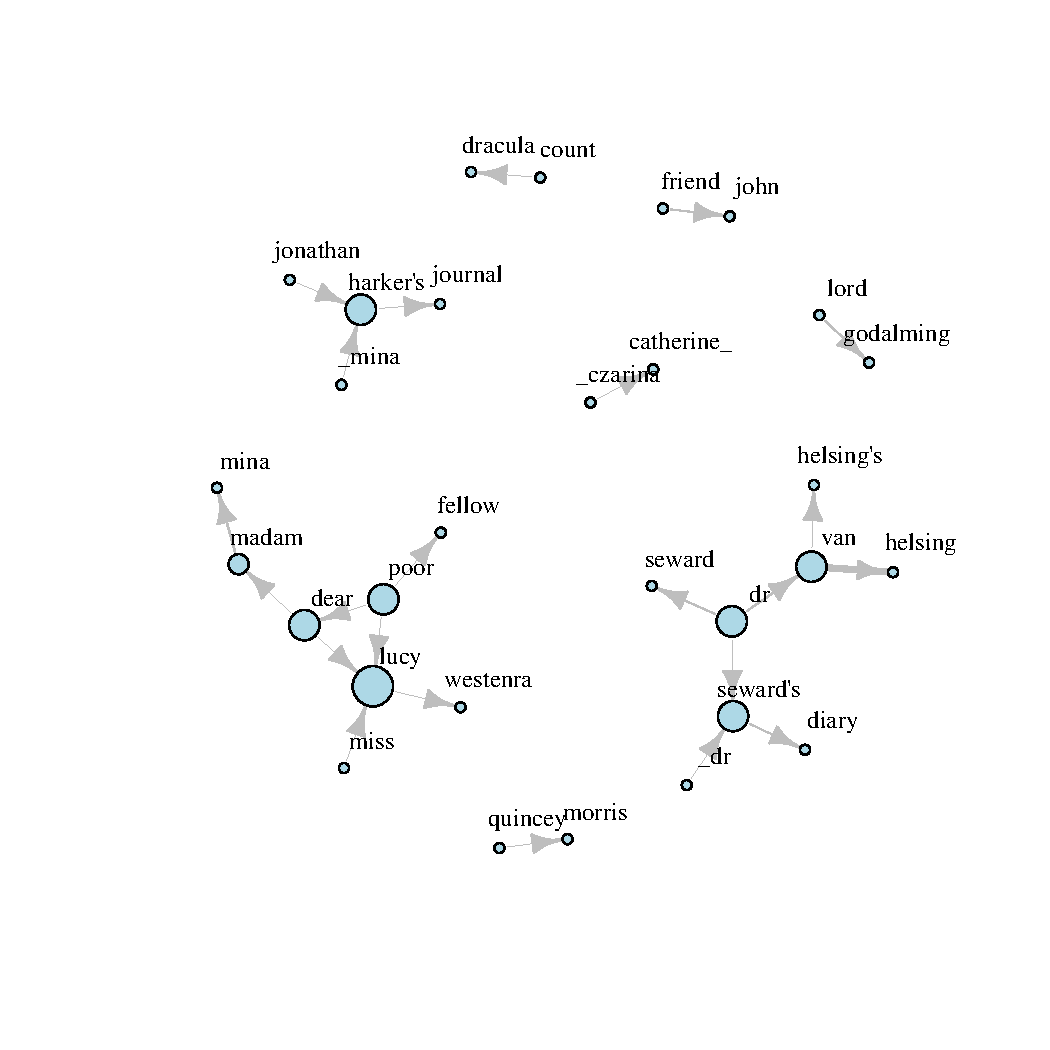
\includegraphics[width=1\textwidth]{bigramas.pdf}
    \caption{Grafo de bigramas más representativos en la obra \textit{Dracula}. Los vértices dirigidos representan la secuencia de los bigramas y el tamaño de los nodos el conteo de cada palabra utilizada en los bigramas.}
    \label{bigramas}
\end{figure}

\bibliographystyle{plainnat}
\bibliography{Biblio}

\end{document}